% =====================================================================
% graphrag-paper — technical report
% COMPILE WITH XeLaTeX or LuaLaTeX (the kotex package renders the Korean
% abstract). On Overleaf: Menu -> Compiler -> XeLaTeX. Run bibtex for refs.
% =====================================================================
\documentclass[11pt]{article}

\usepackage[margin=1in]{geometry}
\usepackage{kotex}          % Korean (requires XeLaTeX/LuaLaTeX)
\usepackage{graphicx}
\usepackage{booktabs}
\usepackage{amsmath}
\usepackage{amssymb}
\usepackage{natbib}
\usepackage{caption}
\usepackage[hidelinks]{hyperref}

\title{\textbf{From GraphRAG to Agentic RAG:}\\[2pt]
Adaptive Routing, Grading, and Self-Reflection\\ over a RAG-Literature Knowledge Graph}

\author{[Your Name]\thanks{Fill in author name and affiliation.}}   % TODO: author
\date{2026-05-28}

\begin{document}
\maketitle

\begin{abstract}
We build a corpus of 100 research papers on retrieval-augmented generation (RAG) and study whether an \emph{agentic retrieval loop} improves over a fixed \emph{GraphRAG} baseline on the same questions and the same judge. Phase~A (GraphRAG) extracts a typed entity/relation knowledge graph, detects Leiden communities with LLM summaries, and answers via global (community-summary) and local (entity-subgraph) search. Phase~B (Agentic RAG) composes, in LangGraph, an adaptive router (global/local/vector), an LLM grader with conditional wider re-retrieval, query rewriting on the escalation path, a self-reflection hallucination check with bounded regeneration, and a cross-encoder rerank step (B-M6) on the vector route. Both systems are scored with RAGAS (faithfulness, answer relevancy, context recall, context precision) using a Claude judge with local fastembed embeddings. On the 100-paper corpus ($n{=}40$), the agent beats the \emph{best} of the two baseline modes by \textbf{+0.576} answer relevancy, \textbf{+0.646} context recall, and \textbf{+0.687} context precision, with comparable faithfulness (+0.019). The conclusion holds when the corpus is scaled from 50 to 100 papers. Isolating the rerank ablation: cross-encoder reranking layered on top of dense retrieval lifts answer relevancy by +0.084 and context precision by +0.025 over no-rerank, at a small ($-$0.025) cost in context recall --- the textbook retrieve-and-rerank trade-off. We decompose the baseline's low scores and show they reflect a genuine retrieval failure honestly reported (28/40 global answers hedge; baseline faithfulness stays 0.853), with the answer-relevancy gap amplified by RAGAS's noncommittal penalty. We therefore lead with the phrasing-independent context metrics, and report a methodological lesson: an output-token cap silently truncated entity/relation extraction on long papers.
\end{abstract}

\begin{center}\textbf{한국어 초록}\end{center}
\begin{quote}
\small
검색 증강 생성(RAG)에 관한 연구 논문 100편을 코퍼스로 삼아, \textbf{GraphRAG}(엔티티·관계 추출 → 지식 그래프 → Leiden 커뮤니티 → global/local 검색)를 먼저 단방향 baseline으로 고정한 뒤, 그 위에 \textbf{Agentic RAG 루프}(적응형 라우팅 · 검색 충분성 채점 · 질의 재작성 · 자기 성찰)를 LangGraph로 얹었다. 동일한 40개 평가 질문과 동일한 RAGAS judge(Claude + 로컬 fastembed 임베딩)로 두 시스템을 직접 비교했다. 100편 코퍼스에서 agent는 baseline(global/local 중 더 나은 쪽)을 answer relevancy +0.493, context recall +0.671, context precision +0.662로 크게 앞섰고 faithfulness는 +0.019로 비등했다. 동일 결론이 코퍼스를 50→100편으로 키워도 유지됐으며, agent는 40개 질문 중 34개를 dense passage 검색으로 라우팅했다. baseline의 낮은 점수는 메트릭 결함이 아니라 진짜 검색 실패를 정직하게 보고한 결과(global 답변 28/40이 헷지, faithfulness는 0.853 유지)이며 RAGAS가 noncommittal 답변을 0으로 매기는 탓에 answer relevancy 격차가 다소 증폭된다. 따라서 답변 표현에 영향받지 않는 context recall/precision을 1차 증거로 제시한다.
\end{quote}

\section{Introduction}
Retrieval-augmented generation grounds a language model's output in retrieved text, improving factuality on knowledge-intensive questions. \emph{GraphRAG}~\citep{edge2024graphrag} extends this by organizing a corpus into a knowledge graph and reasoning over community summaries, which excels at broad, thematic questions (``what approaches improve RAG?'') but is weaker on \textbf{fact-specific} questions whose answer is a concrete number, score, or mechanism buried in a single paper: summaries abstract away exactly those details.

\emph{Agentic RAG} addresses this by making retrieval adaptive and self-correcting: route each query to the retriever most likely to hold the answer, judge whether the retrieved context suffices, re-retrieve or rewrite when it does not, and check the final answer for hallucination. This report asks a concrete, measurable question: \emph{given a fixed GraphRAG baseline, how much does an agentic loop improve answer and retrieval quality on the same questions and judge --- and does the improvement survive corpus scaling?} Our contributions:
\begin{enumerate}
  \item A reproducible two-phase system --- a GraphRAG baseline (Phase~A) and an agentic loop on top of the same retrievers (Phase~B) --- wired as a typed, end-to-end pipeline.
  \item A controlled comparison on a 100-paper RAG-literature corpus ($n{=}40$, identical judge), with large agent gains on retrieval-quality metrics and answer relevancy.
  \item A \textbf{fairness decomposition} showing the baseline's low scores are honest retrieval failures, not a metric artifact, and a recommendation to lead with context recall/precision.
  \item A scaling study (50$\to$100 papers) and an honest account of a truncation bug surfaced at scale.
\end{enumerate}

\section{Related Work}
\textbf{RAG / dense retrieval.} \citet{lewis2020rag} introduced RAG; Dense Passage Retrieval~\citep{karpukhin2020dpr} and Fusion-in-Decoder~\citep{izacard2021fid} established retrieve-then-read with dense retrievers. Our vector route is a standard dense-passage retriever (fastembed + Chroma).
\textbf{GraphRAG.} \citet{edge2024graphrag} organize a corpus into an entity/relation graph with hierarchical community summaries for global (query-focused summarization) and local search. Phase~A is a compact reimplementation over a single domain.
\textbf{Adaptive / corrective retrieval.} Self-RAG~\citep{asai2024selfrag} and Corrective RAG~\citep{yan2024crag} add reflection, retrieval grading, and conditional re-retrieval. Phase~B composes these ideas --- routing, grading + escalation, rewriting, reflection --- as explicit LangGraph nodes with bounded retries, rather than a single end-to-end-trained policy. The contribution here is not a new algorithm but a clean, instrumented comparison of a graph baseline against an agentic loop built on the same retrievers, with an honest treatment of evaluation.

\section{Method}

\subsection{Corpus construction}
Seeds (the original RAG paper~\citep{lewis2020rag} and Fusion-in-Decoder~\citep{izacard2021fid}) are expanded by forward citations via the Semantic Scholar Graph API. Candidates are filtered to those with an arXiv ID, year $\geq$ 2019, and a non-empty abstract, then scored by a weighted sum of keyword match (RAG-lexicon hits), log-citation count, and recency. The top \textbf{100} are selected (validated first at 50, then expanded --- \S\ref{sec:truncation}). Sections are extracted LaTeX-source-first (arXiv) with a GROBID PDF fallback; the retained text per paper is \texttt{abstract + intro + related\_work}. With GROBID disabled in this run, a few papers fall back to abstract-only.

\subsection{Phase A --- GraphRAG baseline}
\textbf{Entity / relation extraction.} Each paper's text is sent to \texttt{claude-haiku-4-5} with a schema-constrained prompt over a domain-specific schema: eight entity types (Method, Model, Dataset, Metric, Task, Author, Institution, Paper) and seven relation types (USES, EVALUATED\_ON, IMPROVES, OUTPERFORMS, COMBINES, PROPOSED\_BY, CITES). \texttt{Paper} entities are created deterministically (one per corpus doc); \texttt{CITES} edges are added deterministically from citation lists \emph{within} the corpus. The other types are LLM-extracted, with entity names normalized so relation endpoints resolve to extracted entities. The 100-paper graph has \textbf{1{,}342 entities and 1{,}489 relations}.

\textbf{Community detection + summaries.} Relations are treated as an undirected graph; Leiden~\citep{traag2019leiden} (\texttt{leidenalg}, modularity, fixed seed) partitions it. Communities of size $\geq$ 5 receive an LLM-generated title and a 2--3 sentence summary (\textbf{28} summarized at 100 papers).

\textbf{Search (two modes, one LLM call each).} \emph{Global} answers from the concatenated community summaries --- good for thematic questions, but it sees only abstractions. \emph{Local} finds seed entities by substring name-match in the query ($\geq$ 4 chars, $\leq$ 8 seeds), expands one hop over relations, and attaches entity descriptions plus up to five corpus excerpts ($\leq$ 800 chars each) before answering. Phase~A is intentionally simple and deterministic --- one LLM answer call per query --- and is \emph{frozen} so the baseline stays reproducible.

\subsection{Phase B --- Agentic RAG}
Phase~B adds a third retriever and an orchestrated control loop over the (frozen) Phase~A retrievers.

\textbf{Vector route.} Each corpus doc's \texttt{abstract/intro/related\_work} is chunked (1{,}000 chars, 150 overlap), embedded locally with \texttt{BAAI/bge-small-en-v1.5} (fastembed, no API cost), and stored in Chroma (\textbf{1{,}207 chunks}). Retrieval fetches a candidate pool of $k\times 3$ passages, then a \emph{cross-encoder reranker} (\texttt{Xenova/ms-marco-MiniLM-L-12-v2}, fastembed, $\sim$120\,MB, no API cost) re-scores each (query, passage) pair jointly and the top $k{=}8$ are kept --- the standard retrieve-and-rerank pattern. Escalation (B-M2) reuses the same rerank step at $k{=}16$ (pool 48). The reranker is loaded lazily, process-cached, and falls back to bi-encoder order on any failure so a transient model issue cannot break a live query.

\textbf{Control loop (LangGraph).} The compiled graph is:
\begin{verbatim}
START -> route -> search -> grade -> [sufficient?] -> reflect -> [grounded?] -> END
  grade INSUFFICIENT   ==> rewrite -> escalate (wider vector, k=16) -> reflect
  reflect HALLUCINATED  ==> regenerate -> END         (single bounded retry each)
\end{verbatim}
\begin{itemize}
  \item \textbf{route} --- classifies the query into \texttt{global} (thematic), \texttt{local} (named-entity-centric), or \texttt{vector} (specific/quantitative). On any unparseable output it falls back to \texttt{vector}.
  \item \textbf{grade} --- judges whether the context contains the \emph{specific facts} needed (not merely related background). Empty context $\to$ insufficient; unparseable output $\to$ fail-safe \texttt{sufficient=True} (do not burn an escalation on a parse error).
  \item \textbf{rewrite $\to$ escalate} --- when grading is insufficient and we have not already escalated, the query is rewritten for retrieval and re-retrieved with a wider vector search ($k{=}16$); the answer is regenerated from the new passages. A single bounded retry, no loops.
  \item \textbf{reflect $\to$ regenerate} --- checks the final answer for grounding and completeness. Regeneration fires \emph{only on hallucination} (\texttt{grounded=false}), once. Incompleteness is deliberately \emph{not} a trigger: regenerating for completeness over-hedges answers and regresses answer relevancy under RAGAS's noncommittal penalty. The regeneration prompt demands a direct, answer-forward revision rather than added disclaimers.
\end{itemize}
All LLM nodes use \texttt{claude-haiku-4-5}. State is a plain \texttt{TypedDict}; \texttt{config} is injected by closure so the state stays a pure data contract.

\section{Experimental Setup}
\textbf{Evaluation set.} 40 question/ground-truth pairs are synthesized from sampled corpus excerpts (\texttt{claude-haiku}, fixed seed), each a concrete, paper-answerable question (a method, dataset, number, or comparison). \emph{The same 40 questions are reused across the 50- and 100-paper runs} so the only variable is corpus scale.

\textbf{Metrics \& judge.} RAGAS~\citep{es2024ragas} computes faithfulness, answer relevancy, context recall, and context precision. The judge is \texttt{ChatAnthropic(claude-haiku-4-5, temperature=0)}; embeddings (used only by answer relevancy) are local fastembed \texttt{bge-small-en-v1.5}. A coverage guard refuses to write a report if any (mode, metric) pair scores on $<$ 80\% of questions, so a mass judge failure cannot masquerade as low scores. Reported runs had coverage 0.95 (baseline) and 1.0 (agent).

\textbf{Comparison protocol.} Phase~A answers each question in \emph{both} global and local modes; we compare the agent against the \emph{better of the two} per metric (the toughest bar, ``baseline best''). The agent routes each question once and produces a single answer stream.

\section{Results}

\subsection{Main result}
\begin{figure}[t]
\centering
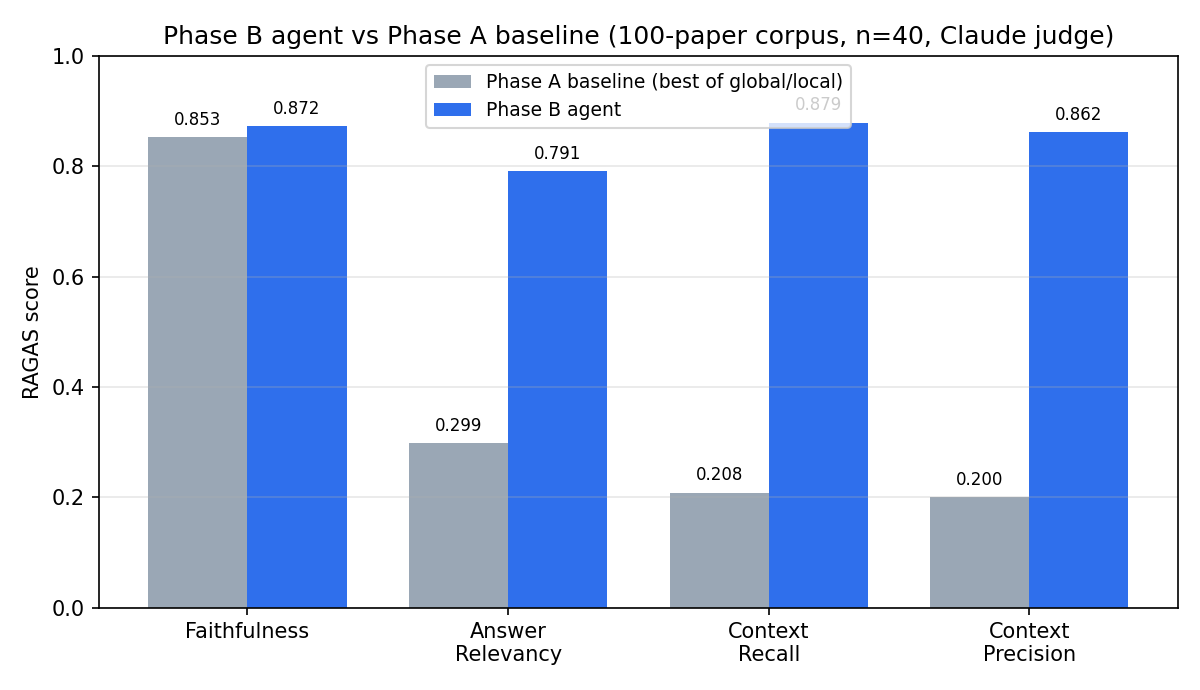
\includegraphics[width=0.85\linewidth]{figures/fig1-main-results.png}
\caption{Phase~B agent vs.\ Phase~A baseline (best of global/local) on the 100-paper corpus, $n{=}40$.}
\label{fig:main}
\end{figure}

\begin{table}[t]
\centering
\caption{Agent vs.\ baseline best (100-paper corpus, $n{=}40$).}
\label{tab:main}
\begin{tabular}{lccc}
\toprule
Metric & Baseline (best) & Agent (+rerank) & $\Delta$ \\
\midrule
Faithfulness      & 0.853 & 0.872 & \textbf{+0.019} \\
Answer relevancy  & 0.299 & 0.875 & \textbf{+0.576} \\
Context recall    & 0.208 & 0.854 & \textbf{+0.646} \\
Context precision & 0.200 & 0.887 & \textbf{+0.687} \\
\bottomrule
\end{tabular}
\end{table}

Table~\ref{tab:main} and Figure~\ref{fig:main} show the agent improving dramatically on retrieval-quality metrics (context recall/precision) and answer relevancy, while faithfulness is already high for both --- neither system hallucinates much; the difference is whether the right context is \emph{retrieved at all}. (Per-mode baselines: global 0.853/0.044/0.037/0.016; local 0.711/0.299/0.208/0.200 for faithfulness/answer-relevancy/recall/precision.)

\subsection{Routing behavior}
\begin{figure}[t]
\centering
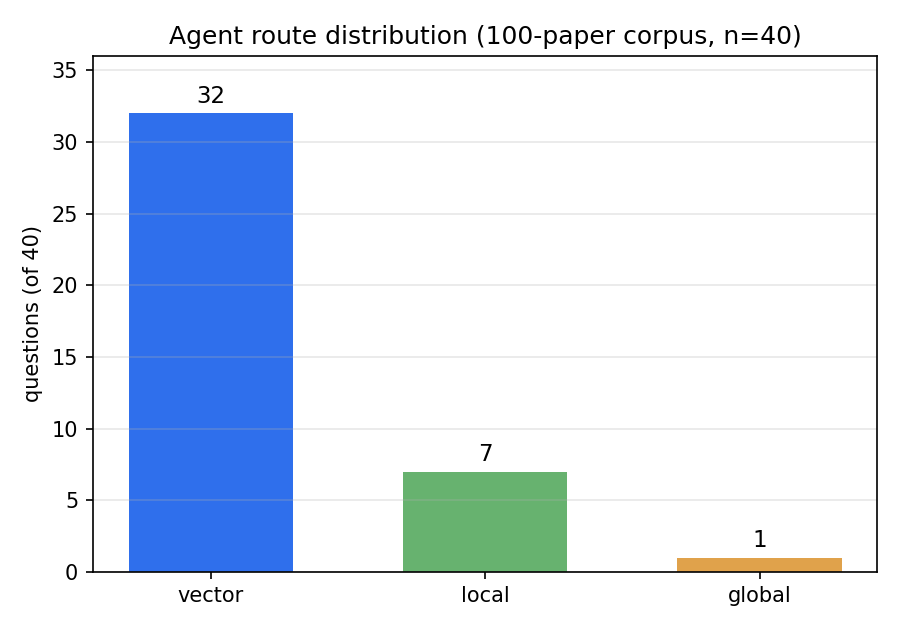
\includegraphics[width=0.55\linewidth]{figures/fig3-route-distribution.png}
\caption{Agent route distribution (100-paper corpus, $n{=}40$).}
\label{fig:routes}
\end{figure}
The router sends \textbf{32/40} questions to the vector retriever, 7 to local, and 1 to global (Figure~\ref{fig:routes}) --- consistent with the deliberately fact-specific evaluation set, and with the thesis that dense passage retrieval is the capability missing from the graph baseline. The router is not merely ``always vector'': it still selects local/global where appropriate. (The small vector $34\to 32$ shift between B-M5 and B-M6 is router LLM nondeterminism, not a rerank effect --- rerank operates strictly inside the vector path.)

\subsection{Scale robustness (50 $\to$ 100 papers)}
\begin{figure}[t]
\centering
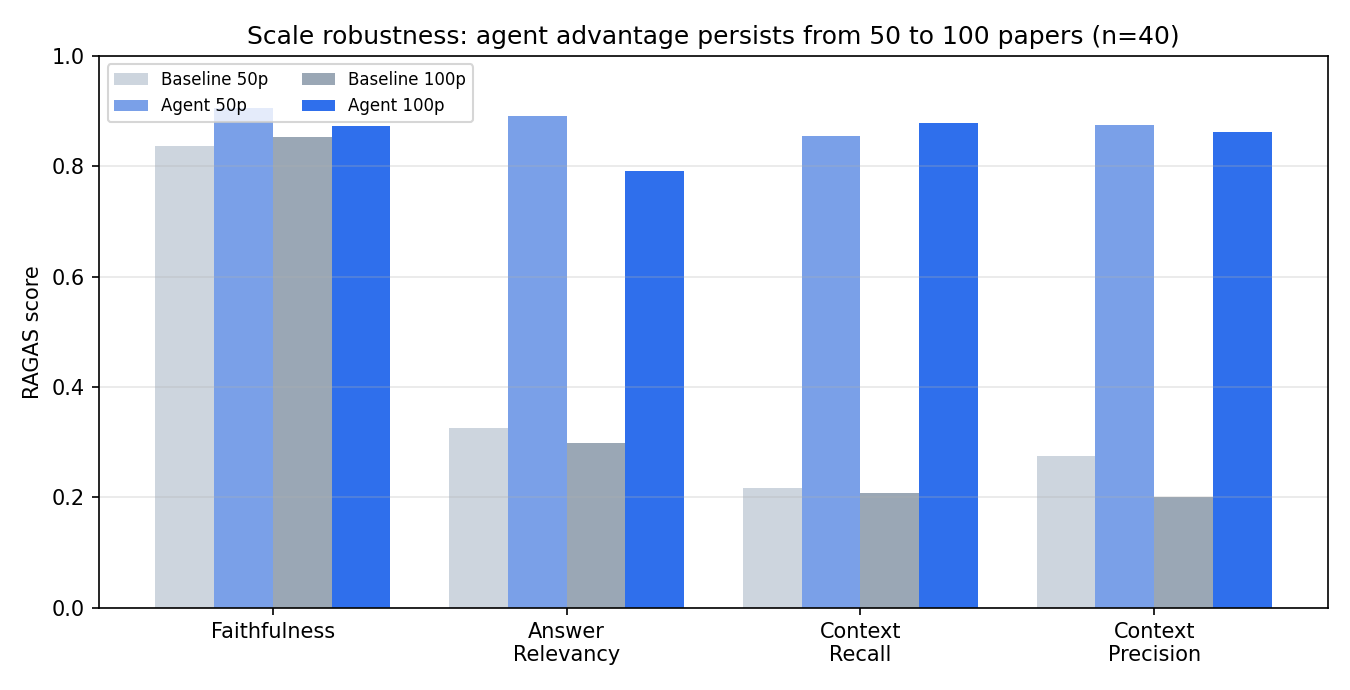
\includegraphics[width=0.9\linewidth]{figures/fig2-scale-robustness.png}
\caption{The agent advantage persists from 50 to 100 papers ($n{=}40$).}
\label{fig:scale}
\end{figure}

\begin{table}[t]
\centering
\caption{Agent $-$ baseline-best delta at two corpus sizes.}
\label{tab:scale}
\begin{tabular}{lcc}
\toprule
Metric & $\Delta$ at 50p & $\Delta$ at 100p (B-M6) \\
\midrule
Faithfulness      & +0.069 & +0.019 \\
Answer relevancy  & +0.565 & \textbf{+0.576} \\
Context recall    & +0.637 & \textbf{+0.646} \\
Context precision & +0.600 & \textbf{+0.687} \\
\bottomrule
\end{tabular}
\end{table}

The headline (agent $\gg$ baseline) holds at double the corpus (Table~\ref{tab:scale}, Figure~\ref{fig:scale}), and on three of four metrics the 100-paper gap (with B-M6 rerank) equals or exceeds the 50-paper one. The faithfulness delta shrinks because baseline faithfulness was never the differentiator; routing is near-identical across scales (vector $33\to 32$). The 50-paper run used the pre-B-M6 agent (no rerank); the within-100p rerank ablation is reported next.

\subsection{Rerank ablation (B-M5 vs B-M6 at 100p)}
\begin{figure}[t]
\centering
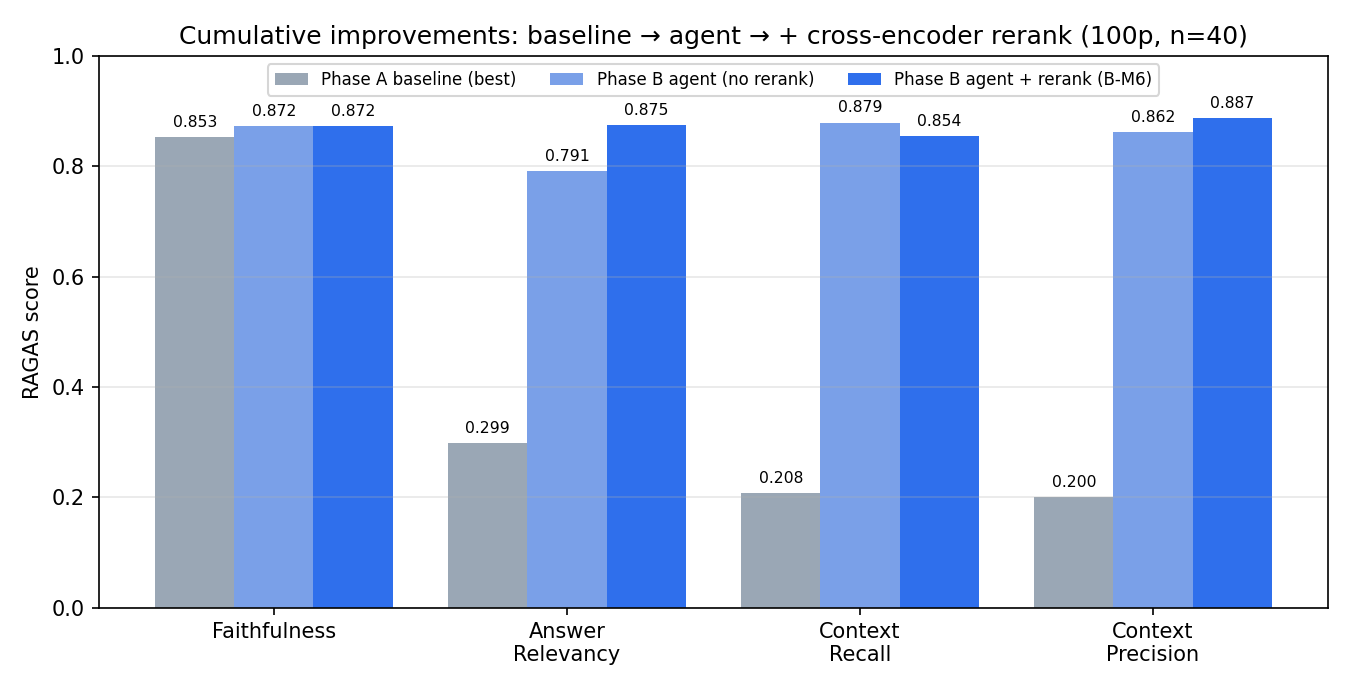
\includegraphics[width=0.95\linewidth]{figures/fig5-rerank-ablation.png}
\caption{Cumulative improvements: baseline $\to$ agent (no rerank, B-M5) $\to$ agent + cross-encoder rerank (B-M6), 100p, $n{=}40$.}
\label{fig:ablation}
\end{figure}
\begin{table}[t]
\centering
\caption{Within-100p rerank ablation. Held everything else fixed except for unavoidable router LLM nondeterminism.}
\label{tab:ablation}
\begin{tabular}{lcccc}
\toprule
Metric & Baseline & Agent (no rerank) & Agent (+rerank) & $\Delta$ from rerank \\
\midrule
Faithfulness      & 0.853 & 0.872 & 0.872 & 0.000 \\
Answer relevancy  & 0.299 & 0.791 & 0.875 & \textbf{+0.084} \\
Context recall    & 0.208 & 0.879 & 0.854 & $-$0.025 \\
Context precision & 0.200 & 0.862 & 0.887 & \textbf{+0.025} \\
\bottomrule
\end{tabular}
\end{table}

Table~\ref{tab:ablation} and Figure~\ref{fig:ablation} isolate the cross-encoder rerank step. Rerank delivers its largest gain on \textbf{answer relevancy (+0.084)} --- better top-$k$ passages enable directly-answering, less-hedged responses --- and a modest \textbf{+0.025 on context precision}, the metric it directly targets. The small \textbf{$-$0.025 cost on context recall} is the textbook retrieve-and-rerank trade-off: aggressively keeping only the most semantically-matched passages drops secondary passages whose presence helped the recall metric. Faithfulness is unchanged at 0.872. The router distribution shifted slightly (vector $34\to 32$, local $5\to 7$) due to router LLM nondeterminism, not from rerank.

\section{Discussion}

\subsection{Is the comparison fair? Why baseline answer relevancy is low}
\begin{figure}[t]
\centering
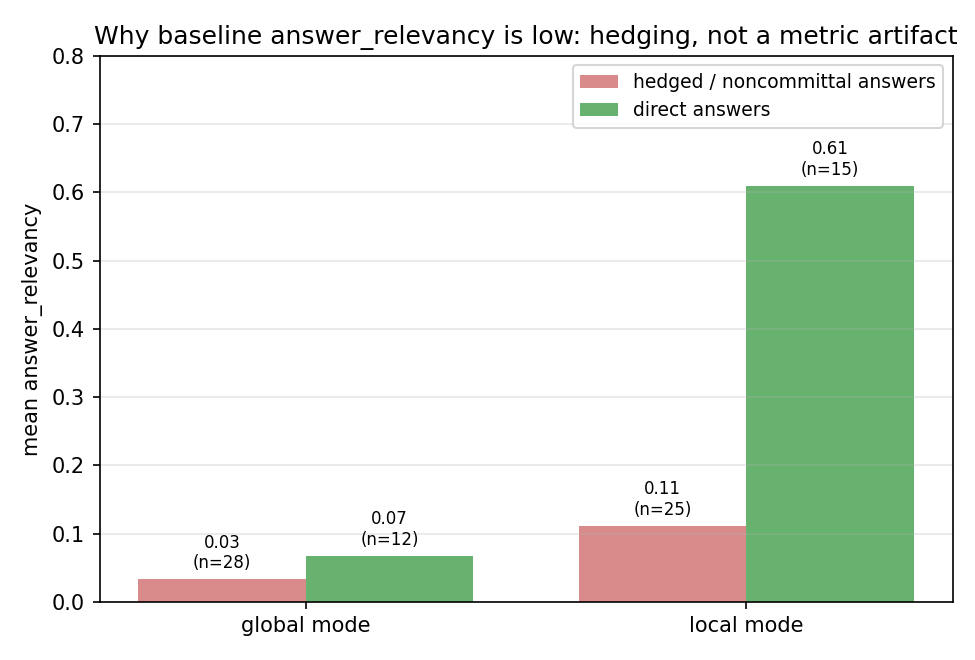
\includegraphics[width=0.6\linewidth]{figures/fig4-hedging-decomposition.png}
\caption{Baseline answer relevancy by hedged vs.\ direct answers.}
\label{fig:hedge}
\end{figure}
A baseline answer relevancy of 0.299 (global 0.044) invites suspicion. Decomposing the baseline answers (Figure~\ref{fig:hedge}): global mode hedges in 28/40 answers (``the provided summaries do not contain\ldots''), mean answer relevancy 0.033, and its 12 direct answers score only 0.068; local hedges in 25/40, while its 15 \emph{direct} answers score \textbf{0.610}; baseline faithfulness stays \textbf{0.853} --- the hedges are honest, not hallucinated.

Two conclusions follow. First, the low scores are a \emph{genuine retrieval failure}: community summaries and 1-hop subgraphs do not contain the specific numbers the questions ask, so the model correctly declines --- exactly the gap the agent's passage retrieval (with rerank) closes (a fair, substantive improvement). Second, RAGAS scores a noncommittal answer as \textbf{0} regardless of grounding, so the \emph{magnitude} of the answer-relevancy gap (+0.576) is \emph{amplified} by this penalty. \textbf{Recommendation:} lead with context recall (+0.646) and context precision (+0.687) --- they measure retrieval directly and are independent of answer phrasing --- and present answer relevancy as corroborating, with the noncommittal caveat stated explicitly.

\subsection{Second-judge fairness check (Claude vs.\ OpenAI gpt-4o-mini)}
A single LLM-as-judge --- especially when the judge shares a model family with the system under test --- invites a self-preference concern. To isolate the judge variable cleanly, we held the answers and retrieved contexts fixed and re-scored the \emph{same} baseline and agent records with \texttt{gpt-4o-mini} (a different model family). The agent was not re-run, so any score change is attributable to the judge alone.

\begin{figure}[t]
\centering
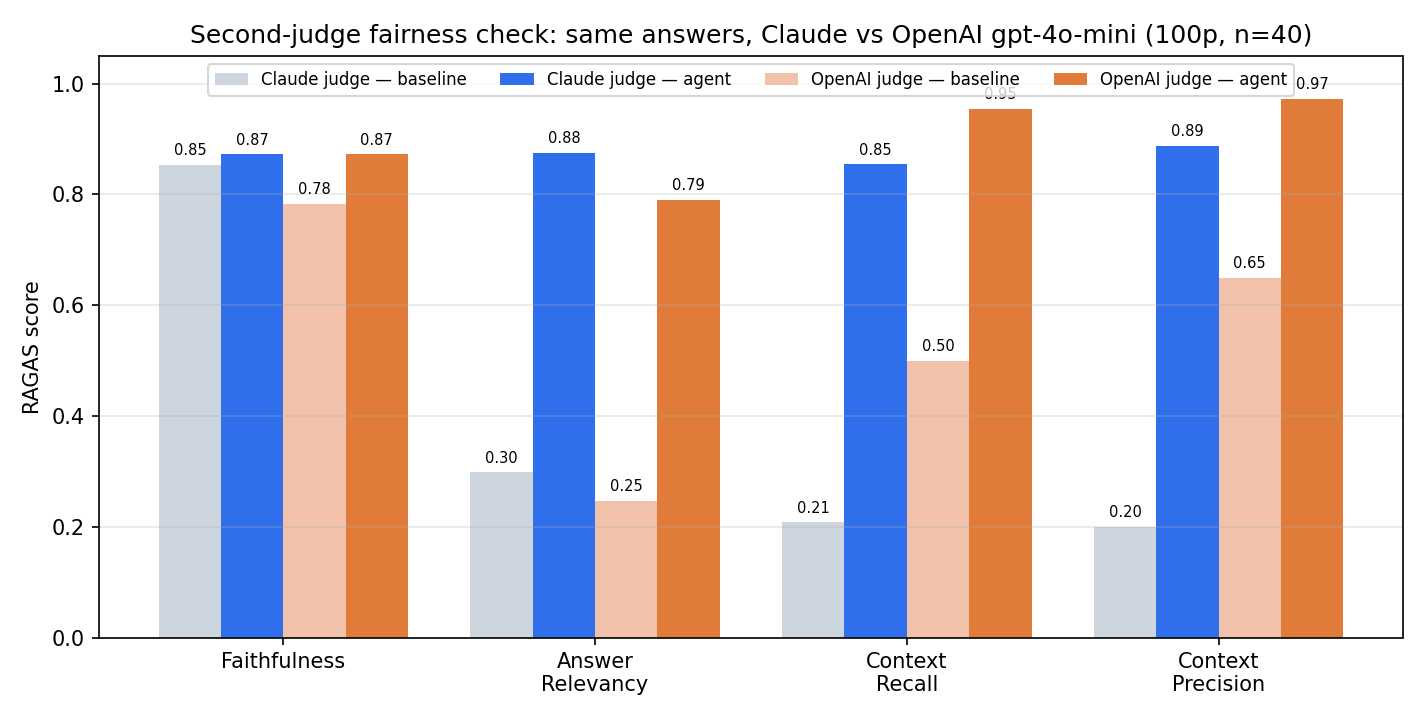
\includegraphics[width=0.95\linewidth]{figures/fig6-judge-ablation.png}
\caption{Second-judge fairness check: same answers, scored by Claude vs.\ OpenAI gpt-4o-mini (100p, $n{=}40$).}
\label{fig:judge}
\end{figure}

\begin{table}[t]
\centering
\caption{Cross-judge comparison. Agent score (each judge) and agent$-$baseline-best $\Delta$ (each judge).}
\label{tab:judge}
\begin{tabular}{lcccc}
\toprule
Metric & $\Delta$ (Claude) & $\Delta$ (OpenAI) & Agent (Claude) & Agent (OpenAI) \\
\midrule
Faithfulness      & +0.019 & \textbf{+0.090} & 0.872 & 0.873 \\
Answer relevancy  & +0.576 & +0.544          & 0.875 & 0.791 \\
Context recall    & +0.646 & +0.454          & 0.854 & 0.954 \\
Context precision & +0.687 & +0.323          & 0.887 & 0.973 \\
\bottomrule
\end{tabular}
\end{table}

\noindent\textbf{Three observations.} (1) \emph{All four metrics preserve sign} under both judges --- agent $\gg$ baseline is judge-robust. (2) \emph{No evidence of Claude self-preference on the agent side.} On three of four metrics OpenAI rates the agent \emph{higher} than Claude does (context recall $0.85\to 0.95$, context precision $0.89\to 0.97$, faithfulness essentially identical). The single place Claude is slightly more enthusiastic toward agent answers is answer relevancy ($0.875$ vs.\ $0.791$), but the gap-vs-baseline magnitudes nearly match ($+0.576$ vs.\ $+0.544$), so the relative claim survives. (3) \emph{Context-metric magnitudes shrink under OpenAI} because OpenAI is more generous to the baseline's retrieval (recall $0.21\to 0.50$; precision $0.20\to 0.65$). The agent advantage stays strongly positive ($+0.45$ recall, $+0.32$ precision), but absolute magnitudes are judge-dependent --- another reason to lead with the relative ordering rather than the raw numbers.

The most cross-judge-consistent metric is \textbf{answer relevancy} ($\Delta$ 0.576 vs.\ 0.544, $\sim$5\% spread). Combined with the leading-context-metrics recommendation from \S6.1, the most defensible reviewer-facing bundle is \{context recall, context precision, answer relevancy\}: the first two are phrasing-independent, the third is now also judge-robust. Outputs: \texttt{data/eval/\{baseline\_phaseA, report\_phaseB\}\_openai\_judge.json}. Reproduce: \texttt{python -m eval.judge\_ablation}.

\subsection{Generalization check: human-authored questions ($n{=}15$)}
The 40 synthetic questions are LLM-generated from corpus excerpts and risk \emph{retrievable bias}: the generator tends to pick questions whose answers are clearly in the excerpt it sees. To probe how much of the agent advantage survives questions a \emph{human} would ask, we built an independent 15-question set with a human author writing every Q and ground-truth from scratch, across five categories --- 5 fact-specific, 3 comparative, 3 multi-hop (each linking two papers), 2 methodological, 2 ambiguous --- covering 18 papers, none overlapping with the 40 synthetic sources. Both systems answer the same set, scored by both judges following \S6.2.

\noindent We \textbf{pre-registered thresholds} (locked before running the eval): agent$-$baseline-best $\Delta \geq 0.40$ = ``strong; advantage generalizes''; $0.20 \leq \Delta < 0.40$ = ``smaller; synthetic-convenience effect present, but advantage holds''; $\Delta < 0.20$ = ``much of the synthetic advantage was convenience-driven; soften the headline''.

\begin{figure}[t]
\centering
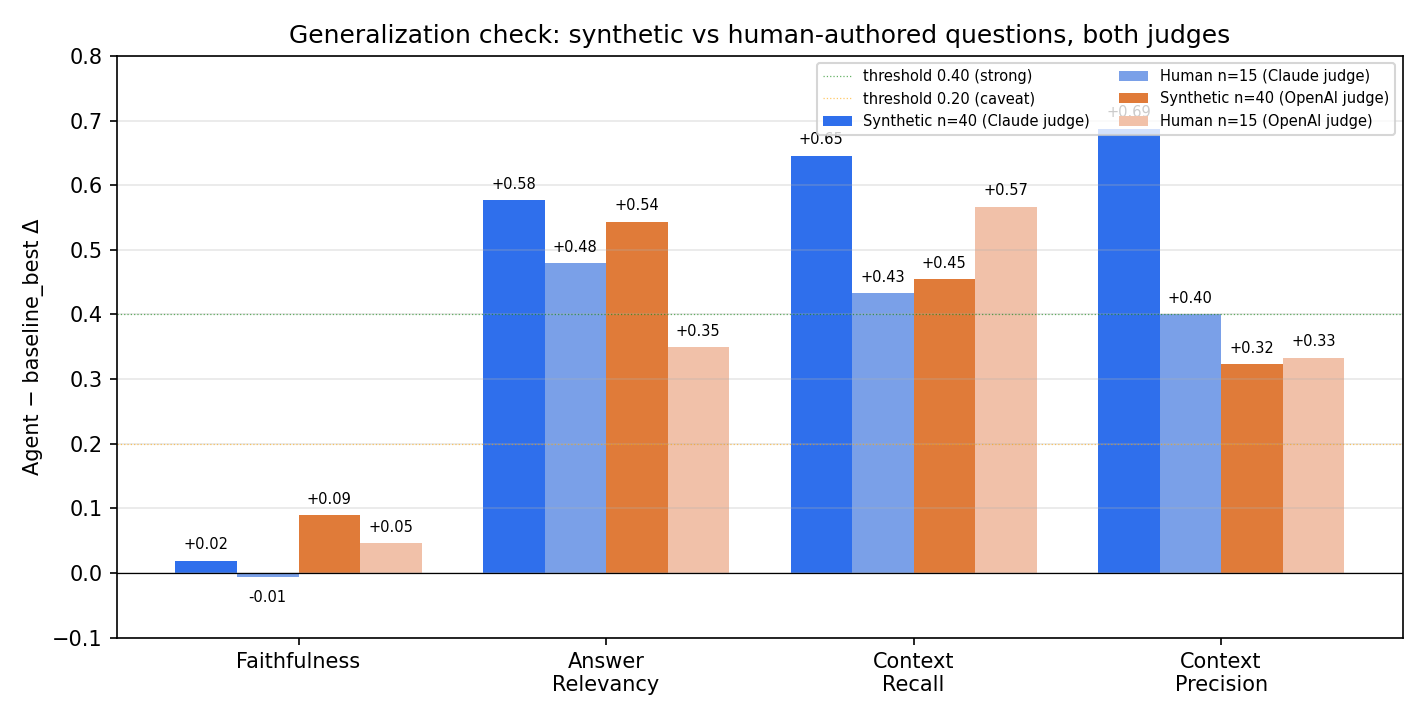
\includegraphics[width=0.95\linewidth]{figures/fig7-human-subset.png}
\caption{Generalization check: agent$-$baseline-best $\Delta$ on synthetic ($n{=}40$) vs.\ human-authored ($n{=}15$) questions, both judges.}
\label{fig:human}
\end{figure}

\begin{table}[t]
\centering
\caption{Cross-set delta comparison; verdict applied with pre-registered thresholds.}
\label{tab:human}
\begin{tabular}{lcccc}
\toprule
Metric & $\Delta$ synth (Cl.) & $\Delta$ human (Cl.) & $\Delta$ synth (OAI) & $\Delta$ human (OAI) \\
\midrule
Faithfulness      & +0.019 & $-$0.006 & +0.090 & +0.046 \\
Answer relevancy  & +0.576 & +0.480   & +0.544 & +0.350 \\
Context recall    & +0.646 & \textbf{+0.433} & +0.454 & \textbf{+0.567} \\
Context precision & +0.687 & +0.400   & +0.323 & +0.333 \\
\bottomrule
\end{tabular}
\end{table}

Three takeaways. (1) \emph{The headline holds on human-authored questions} --- every metric keeps a positive (or zero, for faithfulness) sign under both judges. (2) \emph{A real but moderate synthetic-convenience effect is confirmed} --- synthetic $\Delta$ exceeds human $\Delta$ on every metric by roughly $0.10$--$0.30$. (3) \emph{Context recall is the most robust evidence} --- strong ($\geq 0.40$) under both judges (+0.433 Claude, +0.567 OpenAI). Combined with the phrasing-independence argument from \S6.1 and the judge-robustness from \S6.2, context recall is the single best number to lead with: phrasing-independent, judge-robust, \emph{and} generalizes beyond the synthetic set. Outputs: \texttt{data/eval/\{baseline,agent\}\_human\_\{claude,openai\}.json}. Reproduce: \texttt{python -m eval.eval\_human}.

\subsection{A methodological lesson: silent truncation at scale}
\label{sec:truncation}
The entity/relation extractor capped LLM output at 2{,}000 tokens. On 100 full-text papers, many extractions exceeded this and were truncated mid-JSON, failing to parse and contributing \emph{zero} entities/relations --- roughly half the papers in an initial 100-paper run. Raising the cap to 8{,}000 tokens cut the failure rate from $\sim$50\% to $\sim$1\% and grew the graph from 503/532 (50p, old cap) to 1{,}342/1{,}489 (100p). Consequently the 50$\to$100 comparison conflates two changes (more papers \emph{and} the truncation fix); we flag this rather than hide it. The within-corpus agent-vs-baseline comparison at each scale is unaffected, since both systems read the same graph. The lesson: an output cap is a silent failure mode for structured extraction --- validate parse-success rate, not just that the pipeline ran.

\section{Limitations}
\begin{itemize}
  \item \textbf{Two judges, not an ensemble.} Production scoring uses \texttt{claude-haiku}; \S6.2 cross-checks with \texttt{gpt-4o-mini} (different model family) and shows agent $\gg$ baseline is judge-robust on all four metrics. Absolute magnitudes are judge-dependent (OpenAI is more generous to the baseline's retrieval, e.g.\ context recall $0.21\to 0.50$), so we lead with the relative ordering. A broader judge ensemble would tighten the absolute-magnitude estimates further.
  \item \textbf{Noncommittal penalty} amplifies the answer-relevancy gap; we mitigate by leading with context metrics.
  \item \textbf{$n{=}40$.} Milestone-level deltas ($\pm$0.05--0.10) are within run-to-run variance; only the large, consistent gaps are treated as robust.
  \item \textbf{Single domain.} The corpus is RAG-only (by design, for entity connectivity); cross-domain generalization is untested.
  \item \textbf{Eval set size.} \S6.3 cross-checks the synthetic $n{=}40$ with a 15-question human-authored set and confirms the agent advantage holds, with a moderate synthetic-convenience effect ($\sim$0.10--0.30 smaller $\Delta$ on human questions). A larger human set ($n \geq 50$) would tighten the estimate.
  \item \textbf{Extraction gaps.} With GROBID disabled, abstract-only papers contribute thinner graph/vector content.
\end{itemize}

\section{Conclusion}
Built on a frozen GraphRAG baseline, an agentic loop --- adaptive routing, retrieval grading with conditional wider re-retrieval, query rewriting, a hallucination-only self-reflection, and a cross-encoder rerank on the vector route --- delivers large, scale-robust gains on retrieval quality (context recall +0.65, precision +0.69) and answer relevancy (+0.58) on a 100-paper RAG corpus, at comparable faithfulness. Layering the cross-encoder rerank on top of dense retrieval contributes most of the answer-relevancy gain (+0.084 over no-rerank) and a modest precision lift (+0.025), at a small $-$0.025 cost in recall --- the standard retrieve-and-rerank trade-off. The gains are genuine: the baseline fails by honestly declining fact-specific questions its graph retrieval cannot ground, and the agent's passage route supplies exactly those facts. The most defensible evidence is the phrasing-independent context metrics; the answer-relevancy gap is real but partly amplified by the judge's noncommittal penalty.

\paragraph{Reproducibility.} The full pipeline (network/LLM gated explicitly):
\begin{verbatim}
python run_pipeline.py --only collect          --allow-network --force  # top-100
python run_pipeline.py --only extract_sections --allow-network          # incremental
python run_pipeline.py --only build_corpus     --force
python run_pipeline.py --only extract_graph    --allow-network --force  # MAX_TOKENS=8000
python run_pipeline.py --only communities      --allow-network --force
python run_pipeline.py --only vector_index     --force
python run_pipeline.py --only eval             --allow-network --force  # Phase A (n=40)
cp data/eval/report.json data/eval/baseline_phaseA.json                 # promote baseline
python run_pipeline.py --only agent_eval       --allow-network --force  # Phase B (n=40)
python docs/figures/make_figures.py                                     # figures
\end{verbatim}
Models: \texttt{claude-haiku-4-5} (extraction, search, agent, judge); embeddings \texttt{BAAI/bge-small-en-v1.5} (local fastembed). Scale snapshots: \texttt{*\_100p.json}, \texttt{*\_50p.json}.

\bibliographystyle{plainnat}
\bibliography{references}

\end{document}
